\documentclass{article}

\usepackage{listings}
\usepackage{graphicx}
\usepackage{color} %red, green, blue, yellow, cyan, magenta, black, white
\usepackage{amsfonts}
\usepackage{mathtools}
\usepackage{amsmath}
\usepackage{amssymb}
\usepackage{adjustbox}
\usepackage{hyperref}
\usepackage{float}
\usepackage{caption}
\usepackage{subcaption}
\usepackage[letterpaper, portrait, margin=1in]{geometry}

% % Preamble done! % Begin document
\begin{document}
\label{Cover}
	\begin{center}
	\Large{End-to-end Learning Systems in WiFi Localization}
	\vfill
    Broader Impacts and the Challenges
    \vfill
	Murat Ambarkutuk \\ murata@vt.edu
	\vfill
	Mechanical Engineering Department,\\ Virginia Polytechnic Institute and State University
	\vfill
	\today
	\end{center}
\pagebreak

\section{Indoor Localization}
    Since there is no GPS, so other source of information should be used for localizing the objects.

\section{WiFi Signal in Localization Purposes}
    Since WiFi has become ubiquitious, it started being utilized in different applications varying from customer tracking indoors to robot localization along with communication purposes. % more varying examples would be good.
    However it is available, the information can be extracted from is suffers from being sparse and severely effected by the layouts of environments where WiFi based systems are deployed.
    Thus, it is a great challenge to use this source of information in localization purposes due to the fact that the localization problems require to have higher level of success in localization accuracy and shorter localization time.

\section{Summary of The Proposed System}
    This research proposes a localization system with WiFi signal where a machine learning algorithm is used to infer where the object(s) of interests are in a given environment.
    Similar to the most of the conventional systems proposed earlier, the proposed system is based on the fingerprinting technique where some properties of WiFi signal is obtained in offline stage.
    The collected data are then used for localization during online stage.
    % In offline stage, the signal maps for various WiFi signal sources (Access Points) are constructed via Received Signal Strength (RSS) information and learned by a machine learning algorithm, whereas the online stage contains the proposed localization method based on an information fusion technique.
    The main contribution of this research is that the proposed technique can handle sparse, noisy RSS measurements acquired from the off-the-shelf AP's under LoS and NLoS situations, while achieving comparable localization accuracy to thes state-of-the-art methods by utilizing a state-of-the-art machine learning technique to fully exploit the avaliable information.
    % Another contribution of this system is to fully utilize the collected signals by a Convolutional Neural Network to inherently tackle problems that WiFi systems have to raise, namely, Multipath Effect and noise nature of the WiFi signal.

\section{Broader Impacts}
    The research is mainly focusing on using solely WiFi information to localize the object of interest in an environment.
    Thus, it is important to note that the research does not require any additional hardware than WiFi infrusracture.
    One may realize that this compact design makes it easier to deploy the system various applications with different hardware setups.

    The proposed system, on the contorary to a major part of current research trend, this research requires no additional hardware.
    Two common sensor suits which have been employed for localization problems are LiDAR and cameras.
    However, there are various concerns for these sensors.
    Cameras and LiDARs, for instance, are limited to Line of Sight (LoS) measurements to infer where the sensor suit is located.
    On the other hand, it is possible to extract information with WiFi beyond physical limits where optical sensors cannot, such as behind walls and other obstruction sources.
    Thus, using information from an unconventional source which can extract information beyond such physical contraints would increase our knowledge about the environment.

    Another implication of having no additional sensors is that the system can be easily deploy to variety of hardware infrasracture from embedded devices, Internet-of-Things (IoT) to sophisticated robotic systems.
    For instance, the proposed system can be deployed to drones where the feasibility of operations heavily depend on the payload limits.
    Considering that, LiDAR sensors would not be a good choice for the mentioned example.
    The last implication is that deploying the proposed system in large scale costs significantly lower than the sophisticated sensors would.
    It is typical, for instance, to expect large volume of forklifts in the industrial manufactoring, or product storing area.
    It would cost significantly more to employ LiDAR systems than the proposed system.

    % The proposed system, on the contorary to a major part of current research trend, does not pose any hardware software constrain.
    % In order to,

% \section{The Broader Impacts}
%     The success of the systems relying on the WiFi signal, in general, suffers from the phenomenon called Multipath Effect in which the AP is not in the direct line of sight and the EM waves from the AP where the received signal is propagated through non-line-of-sight, i.e.~concrete and glass walls.
%     Although there is some effort to either model or estimate the Multipath Effect to componsate its effects on the systems~\cite{cai2015identification}, it is still an open problem in the field in order to achieve the same level of success under NLoS observations.
%     %One way to componsate the multipath effect is to find out the first the time epoch the signal is acquired; however, some of these operations require significant change in hardware so that  \# \#.
%     \textit{The proposed system can inherently handle multipath effect, since machine not only can reduce complexity of overall design of the system but also can capture deeper information from the radio maps.}
%     % \textit{More explanation regarding the multipath effect is needed here to emphasize that machine learning algorithms can inherently handle it.}
%
%     Another problem with the WiFi signal which makes it difficult to employ it as the main information source is that the signal acquired is not reliable.
%     Figure~\ref{fig-variance} shows the acquired RSS information acquired with stationary client from the AP's both line-of-sight and non-line-of-sight positions in time.
%     The figure clearly depicts that even for stationary clients, the RSSI readings greatly deviates from the mean in time.
%     % \#\textit{gotta mention that deviation makes it not reliable}.
%     To be able to extract relatively reliable information, some hardware and software changes proposed to incorporate Channel State Information (CSI) provided by Orthogonal Frequency-Division Multiplexing (OFDM) forming WiFi protocol.
%     As~\cite{gao2015channel} suggests/proves, the CSI information provides significantly reliable information.
%     However, to be able to acquire CSI information, a specific type of NIC should be used with a specific type of firmware.
%     This makes it hard to deploy proposed system on Embedded-devices, IoT's and robotic systems.\textit{, while the proposed system can be deployed to almost-any arbitrary system thanks to the simplicity of the design.}
%
%     % \textit{Nail the idea Machine Learning stuff can be deployed practically everywhere}
%
%     The paper is organized as follows.
%     The following section reviews the literature regarding robot localization with WiFi signal.
%     In Sec.~\ref{sec-PF}, we formalize the problem.
%     Section~\ref{sec-SD} thoroughly explains the proposed system.
%     The experimentation and the results are  in Sec.~\ref{sec-EX}.
%     We outline our observation and conclusions in the final section.
\section{The Challenges}
    Even though the WiFi infrasracture is widely available in indoor environments, the information we can extract for the localization is subject to different challenges.
    This section we will address the challenges posed by WiFi signal.

    \begin{figure}[h]
       \centering
      %  \framebox{\parbox{3in}{We suggest that you use a text box to insert a graphic (which is ideally a 300 dpi TIFF or EPS file, with all fonts embedded) because, in an document, this method is somewhat more stable than directly inserting a picture.
      %  }}
       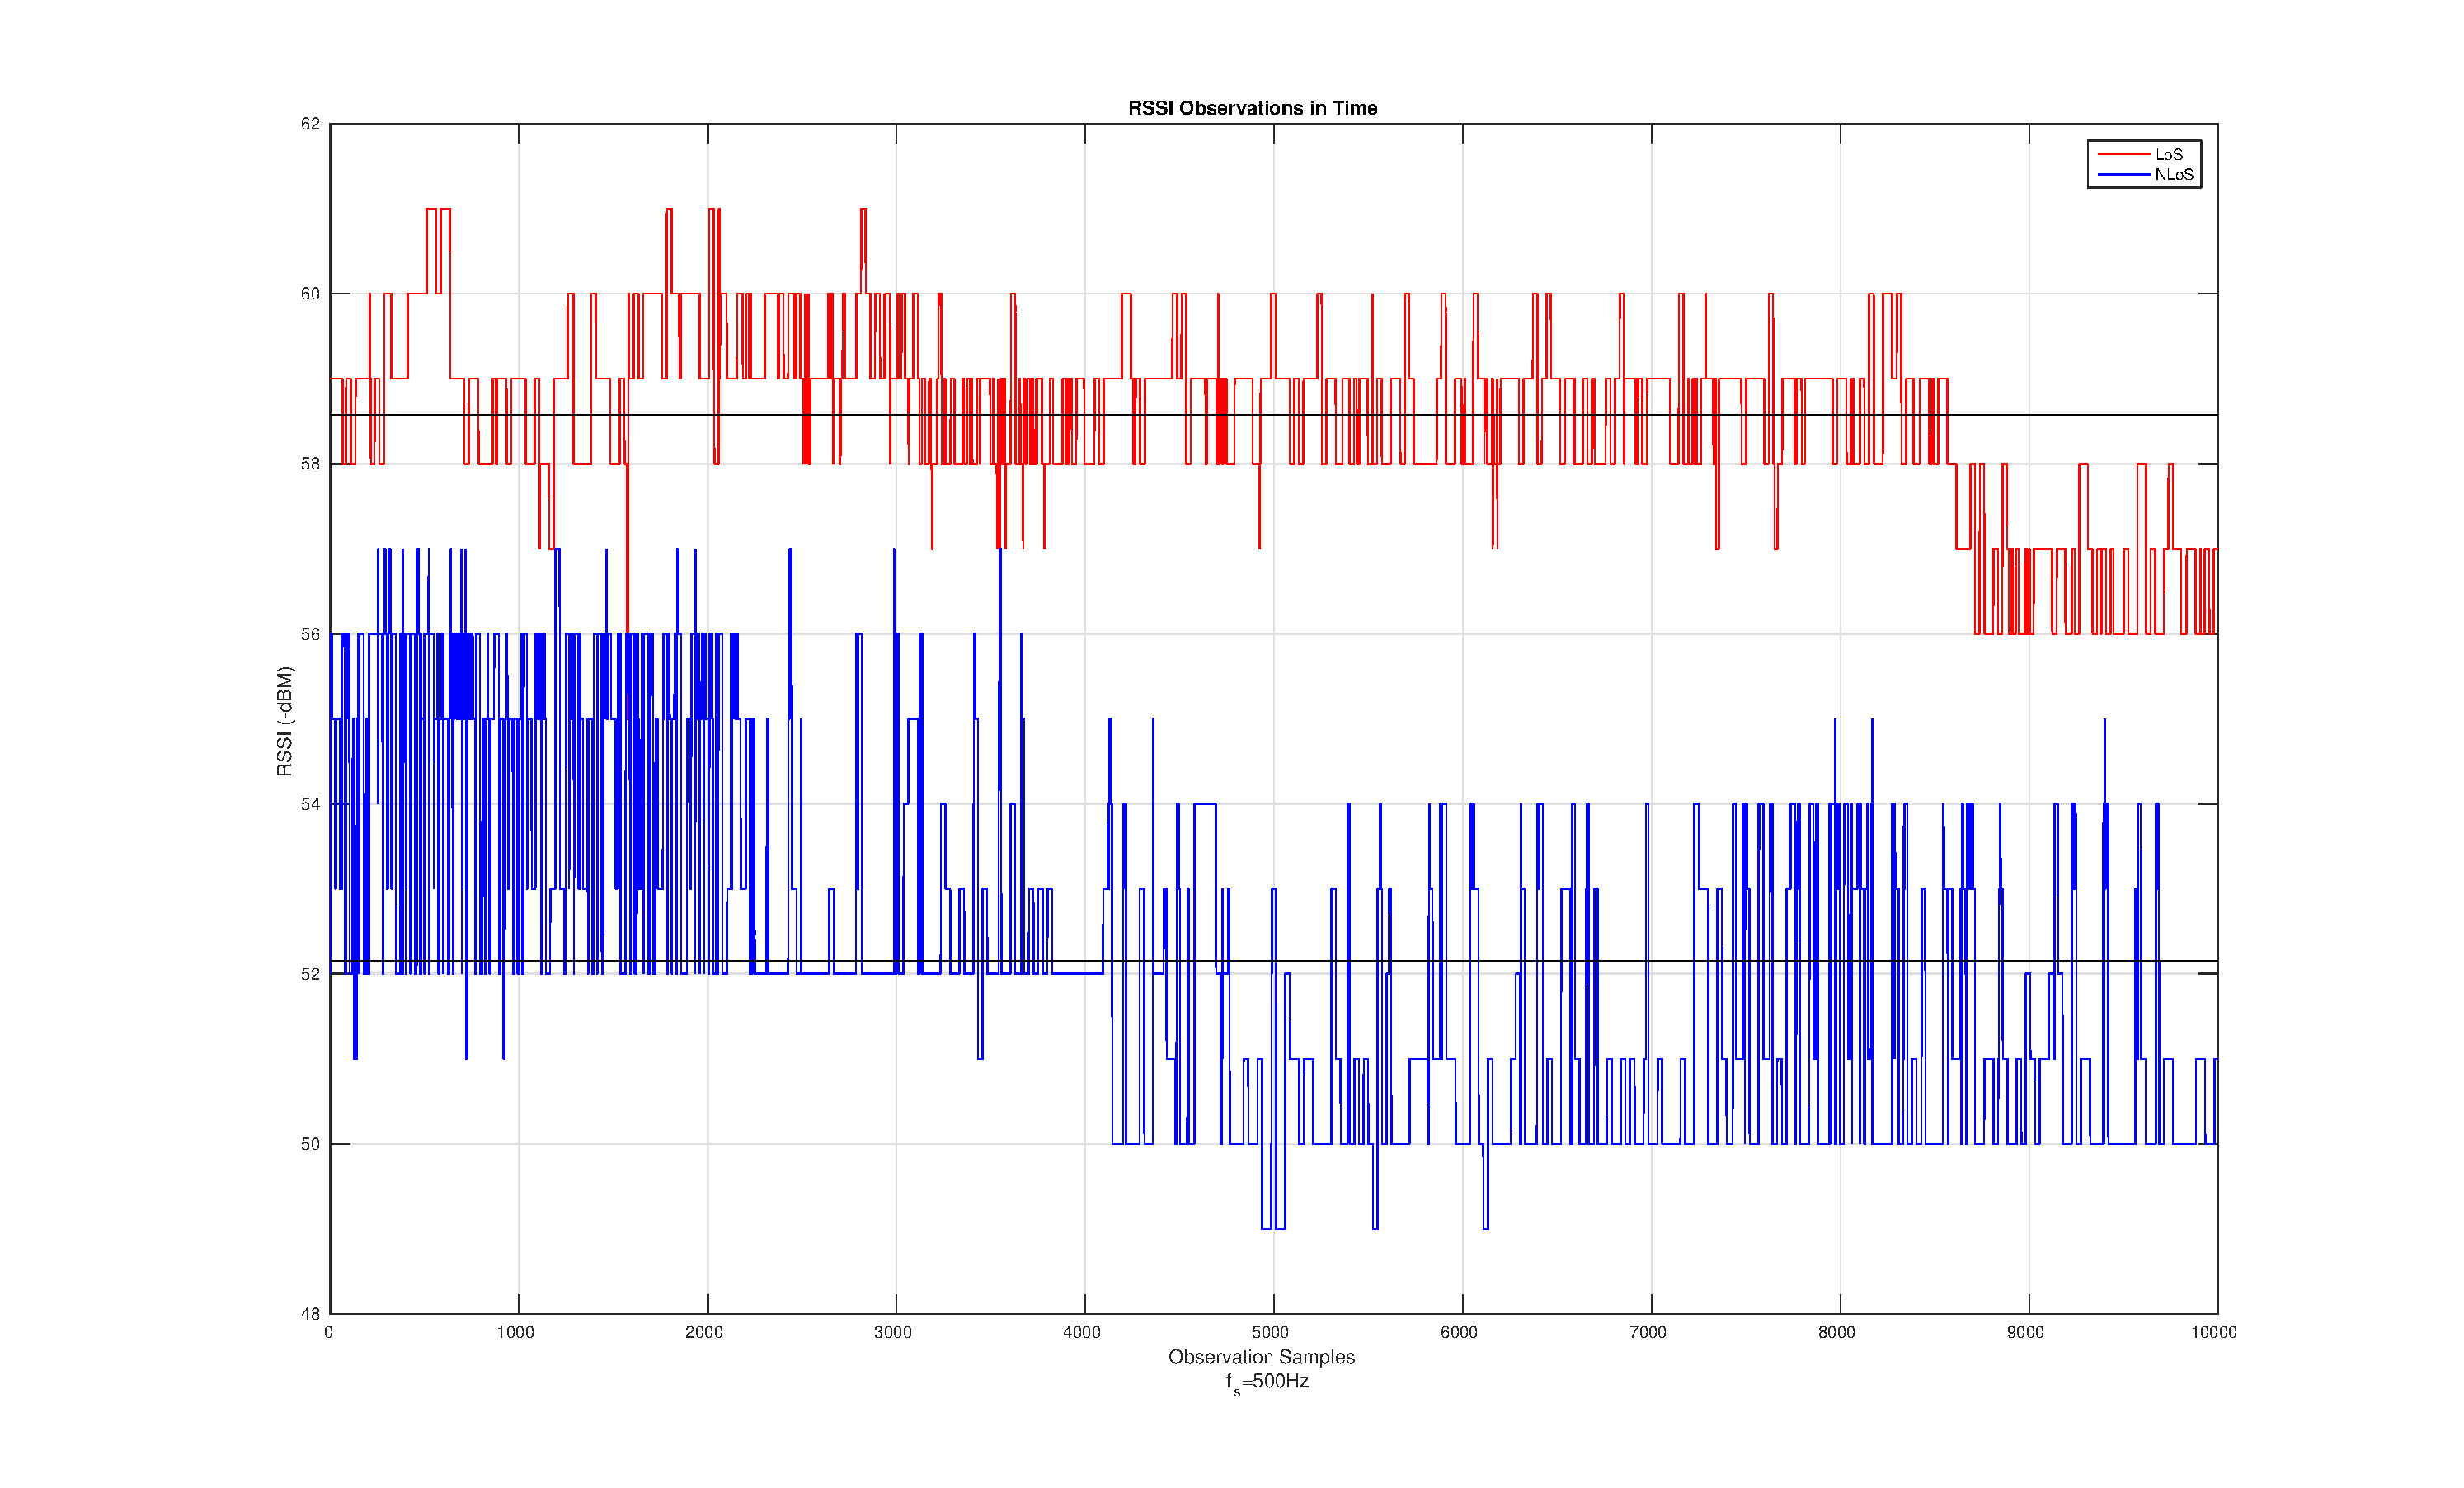
\includegraphics[scale=0.4]{figures/rssi_variance.eps}
       \caption{\label{fig-variance}RSSI readings of NLoS and LoS AP's acquired with a stationary agent}
    \end{figure}

% \bibliographystyle{unsrt}
% \bibliography{bibliography}
\end{document}
